\documentclass{beamer}
\begin{document}
\subsection{Matplotlib}
\begin{frame}[fragile]{Matplotlib}
    \begin{block}{To plot a beautiful line}
        \textbf{matplotlib} is a graphical library specialized in creating interactive and static figures from raw data. 
    \end{block}
    \pause
    \textbf{matplotlib.pyplot}
    \begin{block}{PyPlot}
        \begin{itemize}
            \item \textbf{matplotlib} offer a top-level interfaces, \textbf{pyplot}, to help simplifying figure creation process.
            \item \textbf{pyplot} is designed to provide \textbf{matplotlib} with functions similar to \textbf{MATLAB}.
            \item \textbf{pyplot} states are preserved across multiple functional calls, allowing \textbf{pyplot} to follow the current figure and its changes.
        \end{itemize}
    \end{block}
    more of \textbf{pyplot} at \href{https://matplotlib.org/stable/api/_as_gen/matplotlib.pyplot.html}{matplotlib.pyplot}
\end{frame}
\begin{frame}[fragile]{Matplotlib: Line Plot}
    matplotlib.pyplot.\textbf{plot}([x], y, [fmt], [x2], y2, [fmt2], \dots, **kwargs)\\
    \begin{center}
        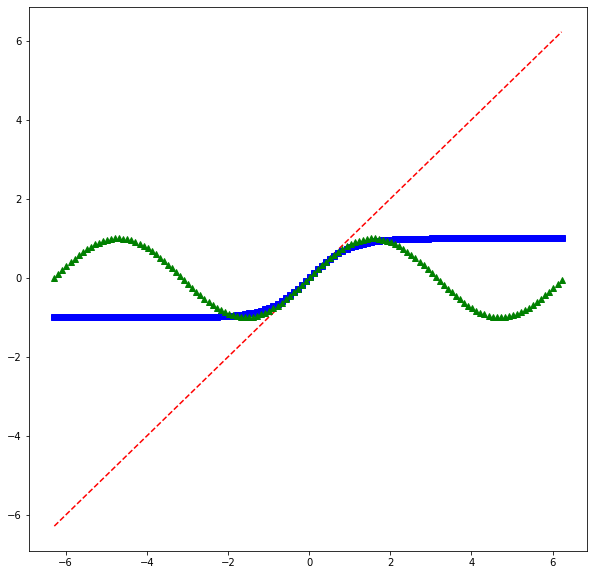
\includegraphics[width=\textwidth,height=0.6\textheight,keepaspectratio]{figures/Plot.png}\\
    \end{center}
    more at \href{https://matplotlib.org/stable/api/_as_gen/matplotlib.pyplot.plot.html}{matplotlib.pyplot.plot}
\end{frame}
\begin{frame}[fragile]{Matplotlib: Plot styles}
    \begin{itemize}
        \item \textbf{Plot styles} consist of 3 elements in combinations: "[marker][line][color]" or [color][marker][line]
        \item For example:
        \begin{itemize}
            \item 'r--' means a red dashed line with no marker.
            \item 'bs' means blue square marker with no line.
            \item 'g\^' means green triangle marker with no line.
            \item 'k:' means a black dotted line with no marker.
            \item 'mX-' means magenta X-filled marker with a solid line.
        \end{itemize}
    \end{itemize}
\end{frame}
\begin{frame}[fragile]{Matplotlib: Scatter Plot}
    matplotlib.pyplot.\textbf{scatter}(x, y, s=None, c=None, marker=None, cmap=None, \dots, **kwargs)\\
    \begin{center}
        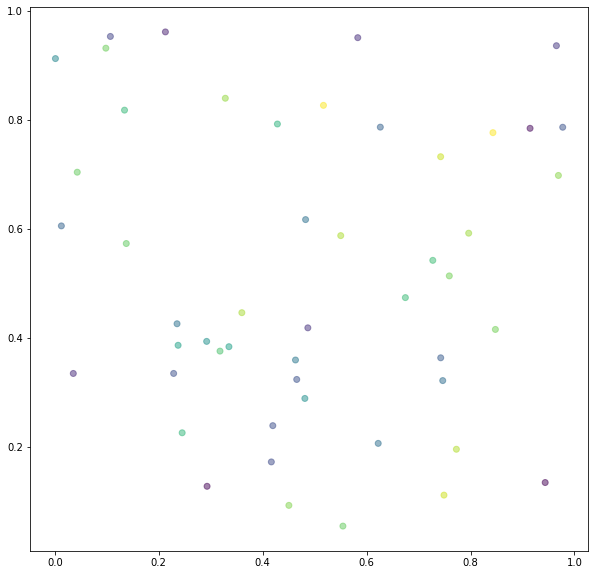
\includegraphics[width=\textwidth,height=0.6\textheight,keepaspectratio]{figures/Scatter.png}\\
    \end{center}
    more at \href{https://matplotlib.org/stable/api/_as_gen/matplotlib.pyplot.scatter.html}{matplotlib.pyplot.scatter}
\end{frame}
\begin{frame}[fragile]{Matplotlib: Box \& Whisker Plot}
    matplotlib.pyplot.\textbf{boxplot}x, vert=None, positions=None, widths=None, patch_artist=None, \dots, **kwargs)\\
    \begin{center}
        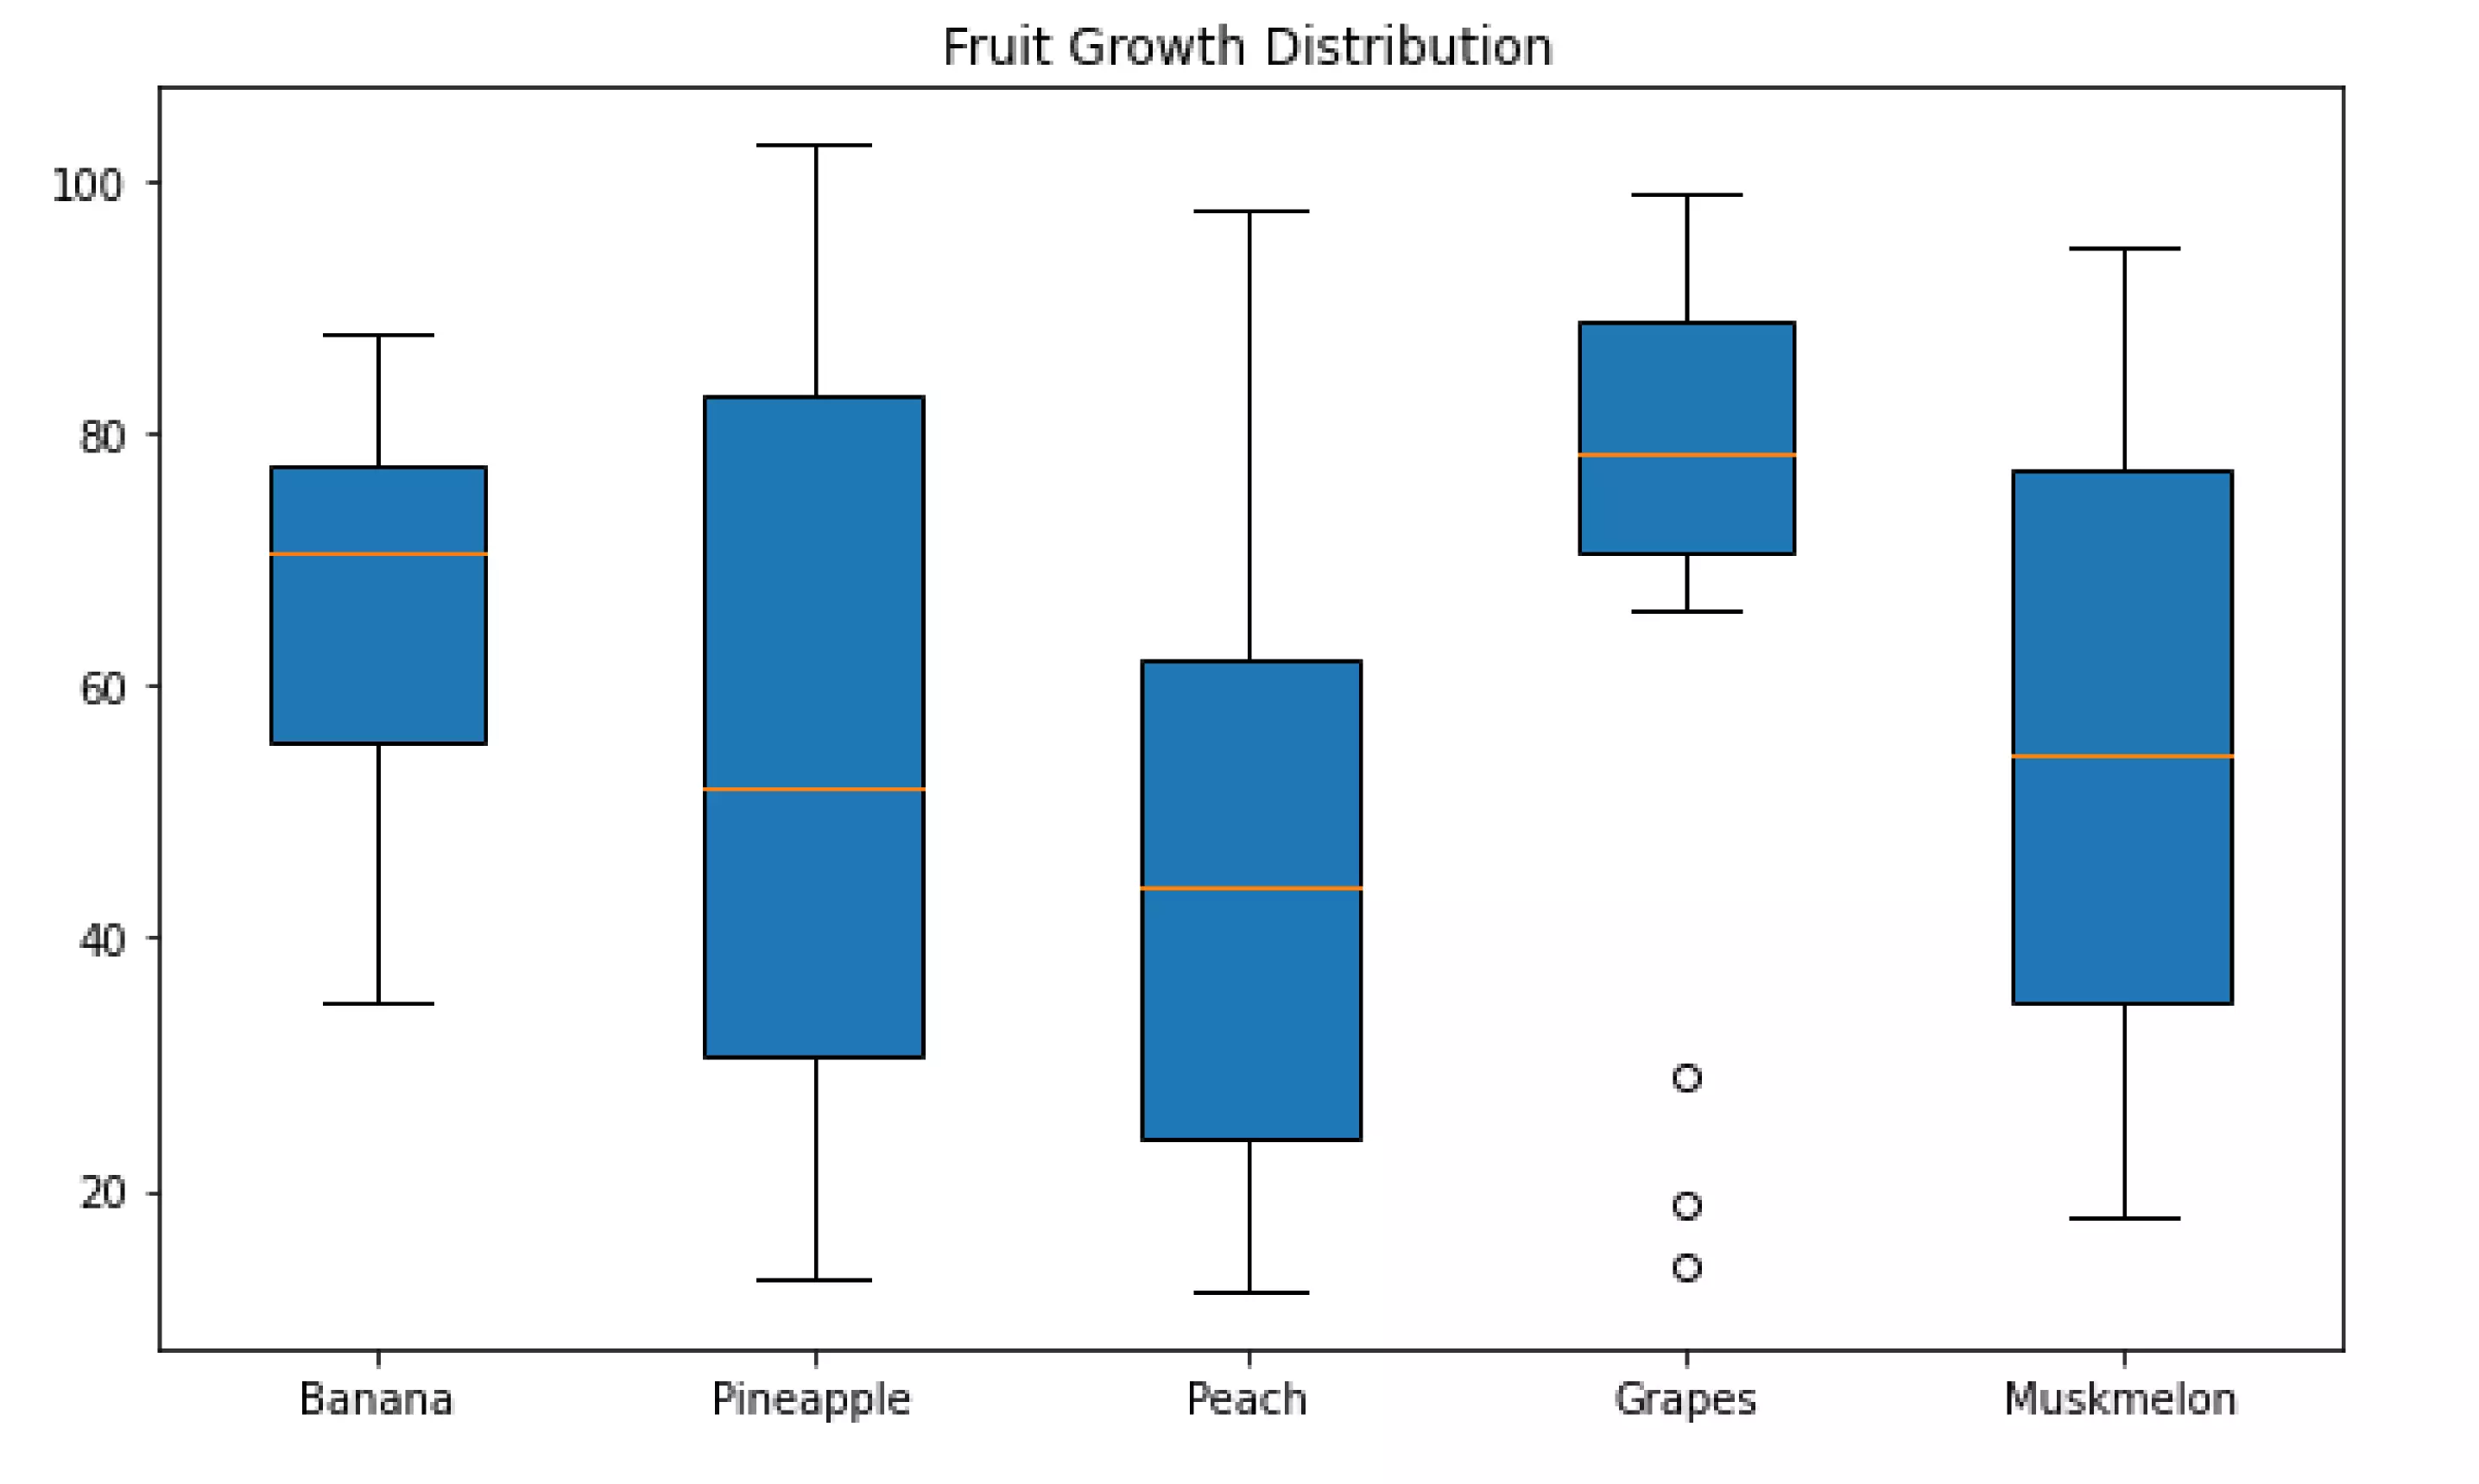
\includegraphics[width=\textwidth,height=0.6\textheight,keepaspectratio]{figures/boxplot.png}\\
    \end{center}
    more at \href{https://matplotlib.org/stable/api/_as_gen/matplotlib.pyplot.hist.html}{matplotlib.pyplot.hist}
\end{frame}
\begin{frame}[fragile]{Matplotlib: Histograms}
    matplotlib.pyplot.\textbf{hist}(x, bins=None, range=None, density=False, \dots, **kwargs)\\
    \begin{center}
        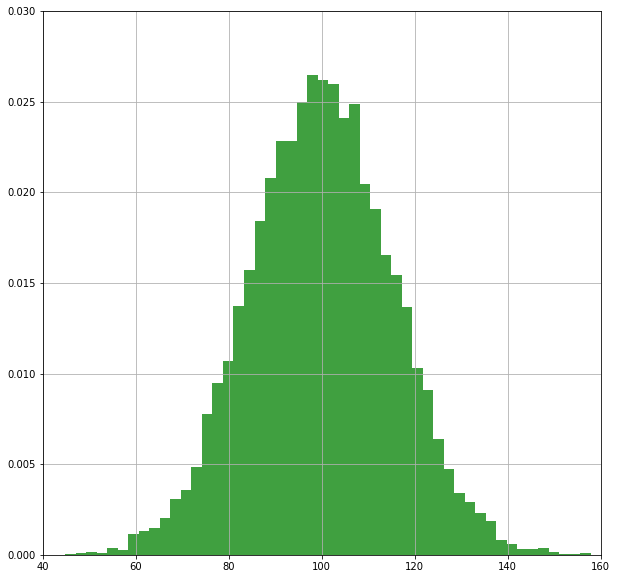
\includegraphics[width=\textwidth,height=0.6\textheight,keepaspectratio]{figures/Hist.png}\\
    \end{center}
    more at \href{https://matplotlib.org/stable/api/_as_gen/matplotlib.pyplot.hist.html}{matplotlib.pyplot.hist}
\end{frame}

\begin{frame}[fragile]
\frametitle{Histograms}
\begin{lstlisting}[language=Python]
# Iterate over the ages and increment
# The corresponding bin count

for age in ages:
    if age < 30:
        bin_counts[0] += 1
    elif age < 40:
        bin_counts[1] += 1
    elif age < 50:
        bin_counts[2] += 1
    else:
        bin_counts[3] += 1

# Create a bar chart of the bin counts

plt.bar(bin_edges[:-1], bin_counts, width=10)
\end{lstlisting}
\end{frame}

\begin{frame}[fragile]
\frametitle{Histograms}
\begin{lstlisting}[language=Python]
# Add labels and a title

plt.xlabel("Age")
plt.ylabel("Count")
plt.title("Age Distribution")

# Show the plot

plt.show()
\end{lstlisting}
\end{frame}

\begin{frame}
\frametitle{Histograms}
\begin{center}
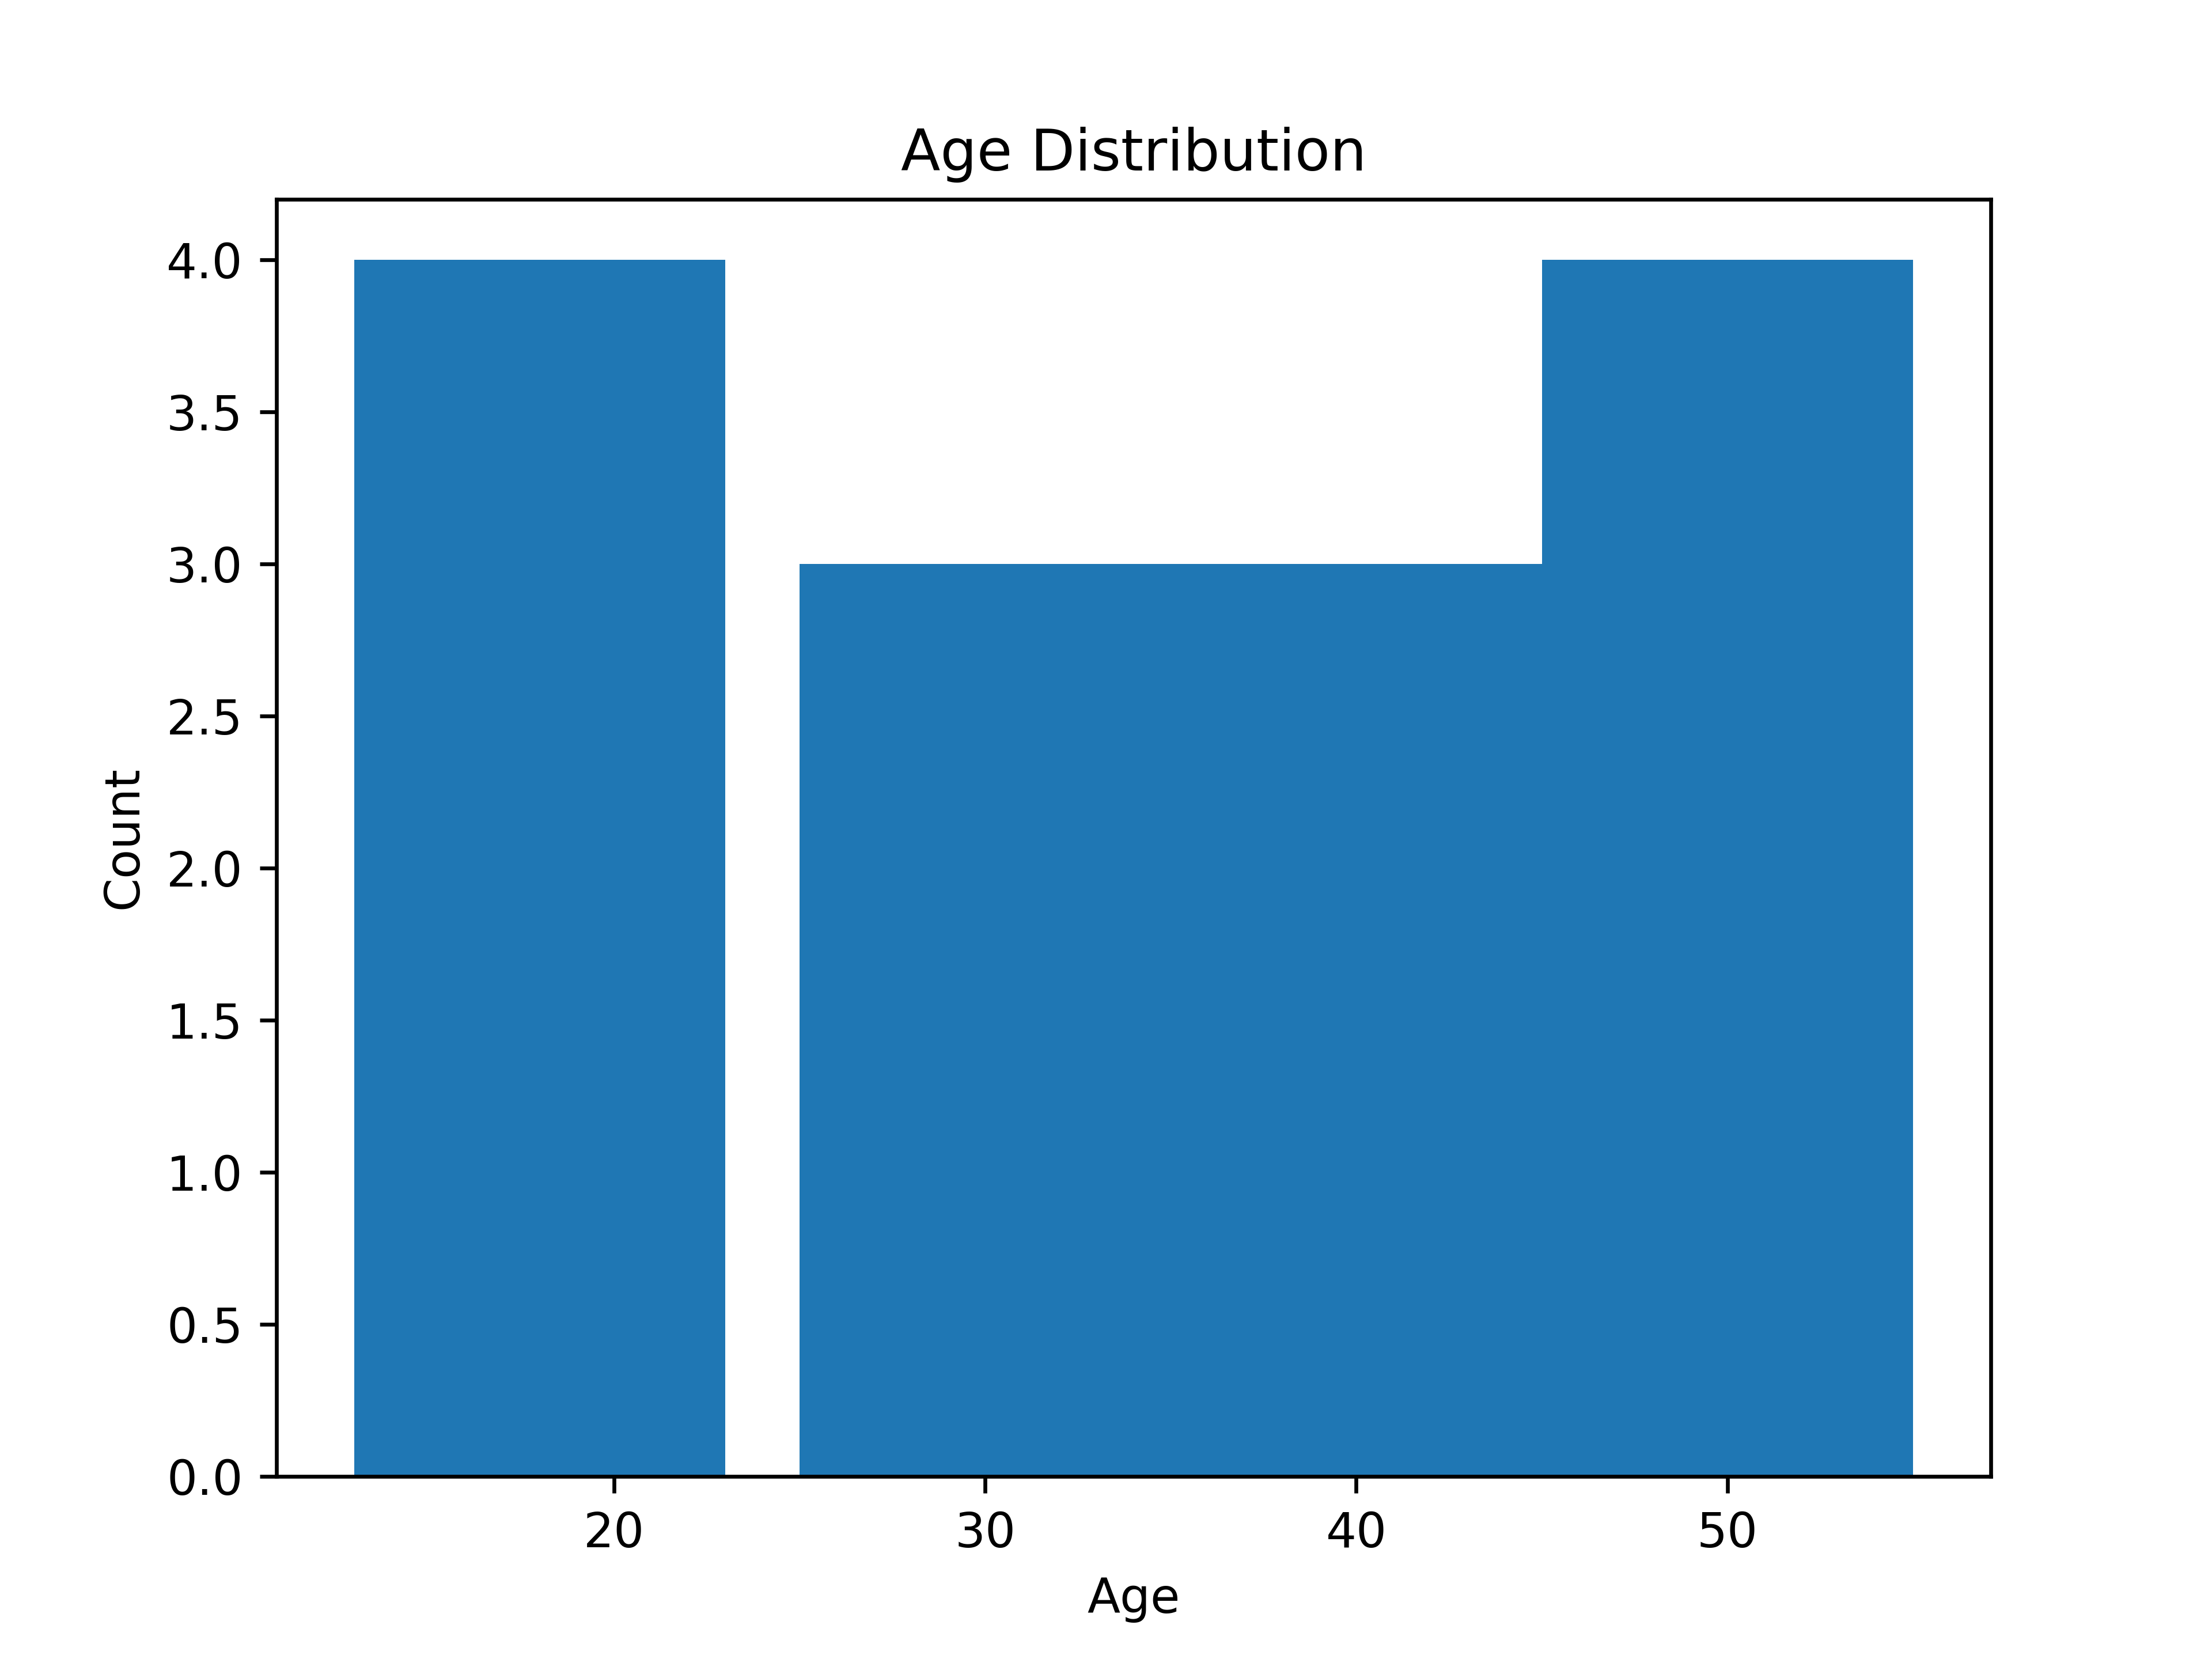
\includegraphics[width=0.7\linewidth]{figures/histogram_example_custom}
\end{center}
\end{frame}

\begin{frame}[fragile]
\frametitle{Box Plots}
\begin{lstlisting}[caption=Creating box plots of data in each column using Pandas and Matplotlib][language=Python]
import matplotlib.pyplot as plt

data.boxplot(column=['Column1', 'Column2', 'Column3'])
plt.ylabel('Value')
plt.title('Box Plots of Columns')
plt.show()
\end{lstlisting}
\end{frame}
\end{document}